\documentclass[journal]{IEEEtran}

\usepackage{comment}
\usepackage{caption}
\usepackage{subfigure}
\usepackage{graphics}
\usepackage{balance}
\usepackage{amsmath}
\usepackage{graphicx}
\usepackage{algorithmic}
\usepackage{array}
\usepackage{url}
\hyphenation{op-tical net-works semi-conduc-tor}

\begin{document}

\title{Topic Modeling}

\author{Balavenkat Gottimukkala\textsuperscript{*}, 
        Pulkit Verma\textsuperscript{+},
        and~Tejas Ruikar\textsuperscript{\$}% <-this % stops a space
\thanks{All authors are associated with Arizona State University, Tempe,
AZ, 85081 USA e-mail: \textsuperscript{*}bgottim1@asu.edu, \textsuperscript{+}pverma13@asu.edu, \textsuperscript{\$}truikar@asu.edu}% <-this % stops a space
\thanks{Final project generated submitted on December 01, 2018.}}

\maketitle

\begin{abstract}
In this paper, we present the design and implementation of a solution to the problem of modelling annotated data. We specifically target data with multiple types where an instance of one type of data serves as a description of another. We describe a hierarchical probabilistic mixture model correspondence latent Dirichlet allocation - that allows for variable representations to be associated with topics.  We have used Gibbs sampling technique to perform posterior inference on the model. We then conducted experiments on 3 different datasets, assessing the models' performance in terms of caption perplexity. Each dataset is made of pairs of data, one datatype being the images in the form of their features other being their respective captions.
\end{abstract}

\begin{IEEEkeywords}
topic modeling, LDA, latent variable, annotated images, Gibbs sampling
\end{IEEEkeywords}
\IEEEpeerreviewmaketitle

\section{Introduction}
\IEEEPARstart{M}{odern} multimedia documents are generally collections of related text, images, audio, and cross-references. There is a lot of yield in using a representation that can model associations among the different data types. Here, we consider a probabilistic model for documents that have a pair of data streams focusing mainly on problems wherein one data type can be considered as an annotation for another data type. The most prominent example is images and their annotations, and this document shows the results of experiments conducted upon that kind of data.

When problems related to annotation are considered, the general objective would be to find the conditional relationship between the two data types. In particular, the task of annotating an unannotated image can be viewed formally as a classification problem—for each word in the vocabulary we must make a yes/no decision. Standard discriminative classification methods, however, generally make little attempt to uncover the probabilistic structure of either the input domain or the output domain. This seems ill-advised in the image/word setting—surely there are relationships among the words labeling an image, and these relationships reflect corresponding relationships among the regions in that image. 

Considering those issues in mind, in this project we try to implement CORR-LDA \cite{corr-lda}, a model that can identify conditional relationships between sets of image regions and sets of words. The model is tested over the Corel-5K data-set and it reveals that this model succeeds in providing an effective conditional relationship model for the annotated images data-sets.

We further extended our experiments onto two other datasets to evaluate the model’s performance. The details of each of the datasets used in the experiments have been provided in the further sections. Section 2 gives the details of few of the previous works related to topic modeling and corr – LDA. Section 3 describes the method and implementation of the model that we have used. Section 4 describes the experiments that we have conducted and gives a brief description of the datasets that we have used. In Section 5, we have all the results that we have obtained after conducting our experiments. Section 6 states our conclusion about this work and finally, Section 7 mentions the future work that is possible and the extensions that can be worked upon.
 
\section{Related Work}
Most of initial methods used in probabilistic modeling of multi-type data used a \textit{Gaussian-multinomial mixture} model \cite{barnard2003matching,shi2000normalized} (GM-Mixture). In this model, a single latent variable is used to represent the joint clustering of both kinds of data. A basic problem with such an approach is that we cannot always assume that the underlying factors are the same for both kinds of data. 

The \textit{Latent Dirichlet allocation} \cite{blei2003latent} model resolved this problem by allowing the latent factors to come from separate distributions. This provided significant improvements over simple mixture models \cite{corr-lda}. However, according to \cite{corr-lda}, ``good models of joint probabilities of images and captions do not necessarily yield good models of conditional probabilities needed for automatic labeling, text-based image retrieval, and region labeling". This was attributed to the absence of dependency between the latent variables of both data types. 

CORR-LDA  solves this problem by combining the flexibility of GM-LDA and associativity of GM-Mixture. It provides with a model for conditional distribution which results into annotation of the data.

\section{Method}
\subsection{Correspondence LDA}
\begin{figure*}
    \centering
    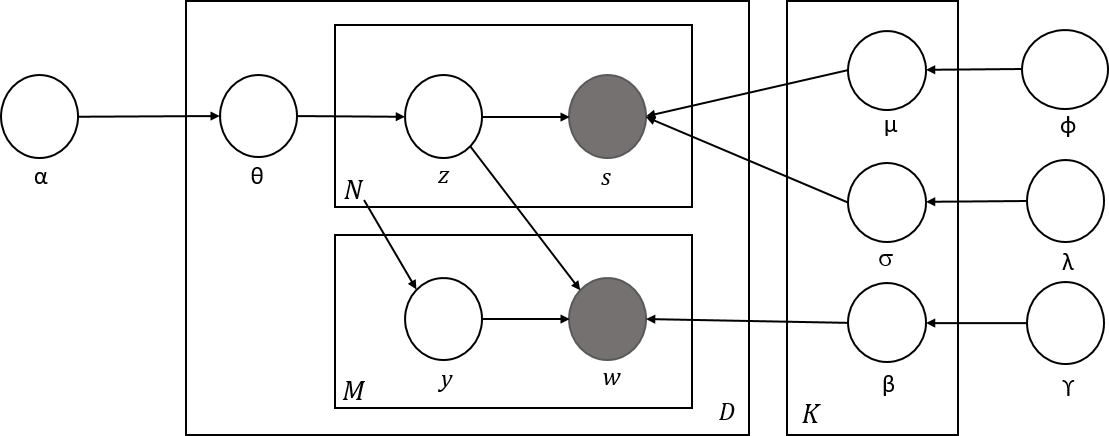
\includegraphics[width= 0.7\textwidth]{images/corrLDA.png}
    \caption{``The graphical model representation of the CORR-LDA model" \cite{corr-lda}}
    \label{fig:corr-lda}
\end{figure*}
Correspondence LDA \cite{corr-lda} was introduced to address the shortcomings of LDA. CORR-LDA can be represented as a probabilistic graphical model as shown in figure \ref{fig:corr-lda}. As a generative method, the CORR-LDA can be used to first generate $N$ SIFT features $r_n$ from an LDA model, and then similar to \cite{corr-lda}, for each of the $M$ caption words, one SIFT feature is selected and a word $w_m$ associated with it is chosen. This $w_m$ is conditioned on the same factor $z$ that generated the SIFT feature. 

Formally, let the latent factors that generate the image be represented as $\mathbf{z} = \{z_1, z_2,\dots,z_N \}$, and the discrete indexing variables be represented as $\mathbf{y} = \{y_1, y_2,\dots,y_M \}$, where $y_i \in \{1..N\}$ and $P(y_i = k) = \frac{1}{N} \, \forall \, k \in \{1..M \} $.

To generate a $K$-factor CORR-LDA model, conditioned on $N$ and $M$, the following process is assumed to generate an image and caption pair $(\mathbf{r},\mathbf{w})$:
 \begin{enumerate}
     \item Sample $\theta \sim Dir(\theta | \alpha)$.
     \item For each image SIFT feature $s_n$, $n \in \{1,\dots,N\}$:
     \begin{enumerate}
         \item Sample $z_n \sim Mult(\theta)$
         \item Sample $s_n \sim p(r|z_n,\mu,\sigma)$ from a Multivariate Gaussian distribution conditioned on $z_n$ .
     \end{enumerate}
     \item For each caption word $w_m$, $m \in \{1,\dots,M\}$:
     \begin{enumerate}
         \item Sample $y_m \sim Uniform(1,\dots,N)$
         \item Sample $w_m \sim p(w|y_m,z,\beta)$ from a multinomial distribution conditioned on the $z_{y_m}$ factor.
     \end{enumerate}
 \end{enumerate}
CORR-LDA specifies the joint distribution on image SIFT features, caption words, and latent variables.

\begin{flalign*}
p(\mathbf{s}, \mathbf{w}, \theta, \mathbf{z}, \mathbf{y}) = p(\theta|\alpha) &\Big( \prod_{n=1}^{N} p(z_n|\theta) p(s_n|z_n,\mu,\sigma) \Big) \\&. \Big( \prod_{m=1}^{M} p(y_m|N)p(w_m|y_m,\mathbf{z},\beta) \Big)    
\end{flalign*} 
 
\subsection{Inference and Estimation}
The Corel-5k dataset consists of words $\mathbf{w} = \{w_1, w_2,\dots,w_M \}$, where each $w_i$ is associated with some image/caption $d_i$. For each image/caption, we have a multinomial distribution over $K$ topics with parameters $\theta^{d_i}$, so for a word in image/caption $d_i$, $P(z_i=j) = \theta_j^{(d_i)}$. Also, the $j^{th}$ topic is represented by a multinomial distribution over $M$ words with parameter $\phi^{(j)}$, so $P(w_i|z_i=j,y_i) = \phi_{w_i}^{(j)}$. A prior distribution is needed over $\theta^{(d_i)}$ to make any prediction about new image/captions. We have Dirichlet prior $\alpha$ on $\theta^{(d_i)}$ since Dirichlet is conjugate prior of multinomial.\\

\textit{Gibbs Sampling}: 
To obtain samples from complicated probability distributions, we can use Markov chain Monte Carlo procedures. Using this, we can draw samples from the Markov chain directly once the Markov chain converges to the target distribution. The assignment of values to the variables being sampled represents a state in the Markov chain. Using Gibbs sampling, we can reach the next state if we sequentially sample all the variables from their distribution, conditioned on all other variables' current values and data. We will be sampling only the assignment of words to topics, $z_i$. Hence our complete probability distribution will be:

\begin{flalign*}
w_i | z_i, y_i, \phi^{(z_i)} &\sim Multinomial(\phi^{(z_i)})\\
s_i | z_i, \mu_i, \sigma_i &\sim Gaussian(\phi^{(z_i)})\\
\phi &\sim Dirichlet(\beta)\\
z_i | \theta ^{(d_i)} &\sim Multinomial (\theta ^{(d_i)})\\
y_i &\sim Uniform(1,\dots,N)\\
\theta &\sim Dirichlet(\alpha)
\end{flalign*}

So the conditional distribution of $z_i$ is given by
\begin{equation}
    P(z_i=j|\mathbf{z}_{-i}, \mathbf{w},\mathbf{s}) \propto P(w_i|z_i=j,\mathbf{z}_{-i},\mathbf{w}_{-i},\mathbf{s}) P(z_i=j|\mathbf{z}_{-i}),
\end{equation}
and
\begin{equation}
    P(z_i=j|\mathbf{z}_{-i}, \mathbf{w},\mathbf{s}) \propto P(s_i|z_i=j,\mathbf{z}_{-i},\mathbf{s}_{-i},\mathbf{w}) P(z_i=j|\mathbf{z}_{-i})
\end{equation}

CORR-LDA \cite{corr-lda} originally implemented inference using variational inference. Gibbs sampling is much better because it can exactly approximate the target distribute if the number of samples increases. There is no such guarantee with variational inference as its outcome is heavily skewed by the choice of bias. The only disadvantage of the MCMC method over variational inference is the computation time. But for small datasets like Corel-5K, MIR Flickr, and ESP game dataset, we can afford to run Gibbs sampling. 

We have used the sampling procedure as described in \cite{gclda}. It was analyzed in \cite{griffiths2004finding} that we need not directly update the values of the parameters $\theta$, $\mu$, $\sigma$, and $\beta$ during inference, because these distributions are “collapsed out” and hence can be estimated directly from the current values of variables \textbf{y}, and \textbf{z}. We have not tested exclusively for convergence as we ran 10000 iterations for updating the values of parameters during the training phase. 

\subsubsection{Model Initialization}
In order to initialize the model, we randomly assign all $z_i$ variables to one of the topics as given by $z_i$ $\sim$ uniform(1,..., T). The values for $y_i$ are then updated to get the initial values. 

\subsubsection{Parameter Update Sequence}
We update the value of $y_i$ by assigning the assignment of $i^{th}$ caption word $w_i$ corresponding to caption of image $d$ to a topic. Similar to \cite{gclda}, ``the update is conditioned on the current vector $\mathbf{z}^{(d)}$ of assignments of peaks to topics in d, and an estimate of each topic’s multinomial distribution over caption words $\beta(t)$".

We then update the value of $z_i$ representing the assignment of $i^{th}$ sift feature of image $s_i$ to a topic. This update is also conditioned on the $\mu$ and $\sigma$ values.

The update equations are derived from the methodology described by equations (1) and (2).


\begin{figure*}[t]
\centering
\subfigure[Varying values of $\alpha$ for Corel-5k dataset]{%
\label{fig:alpha}%
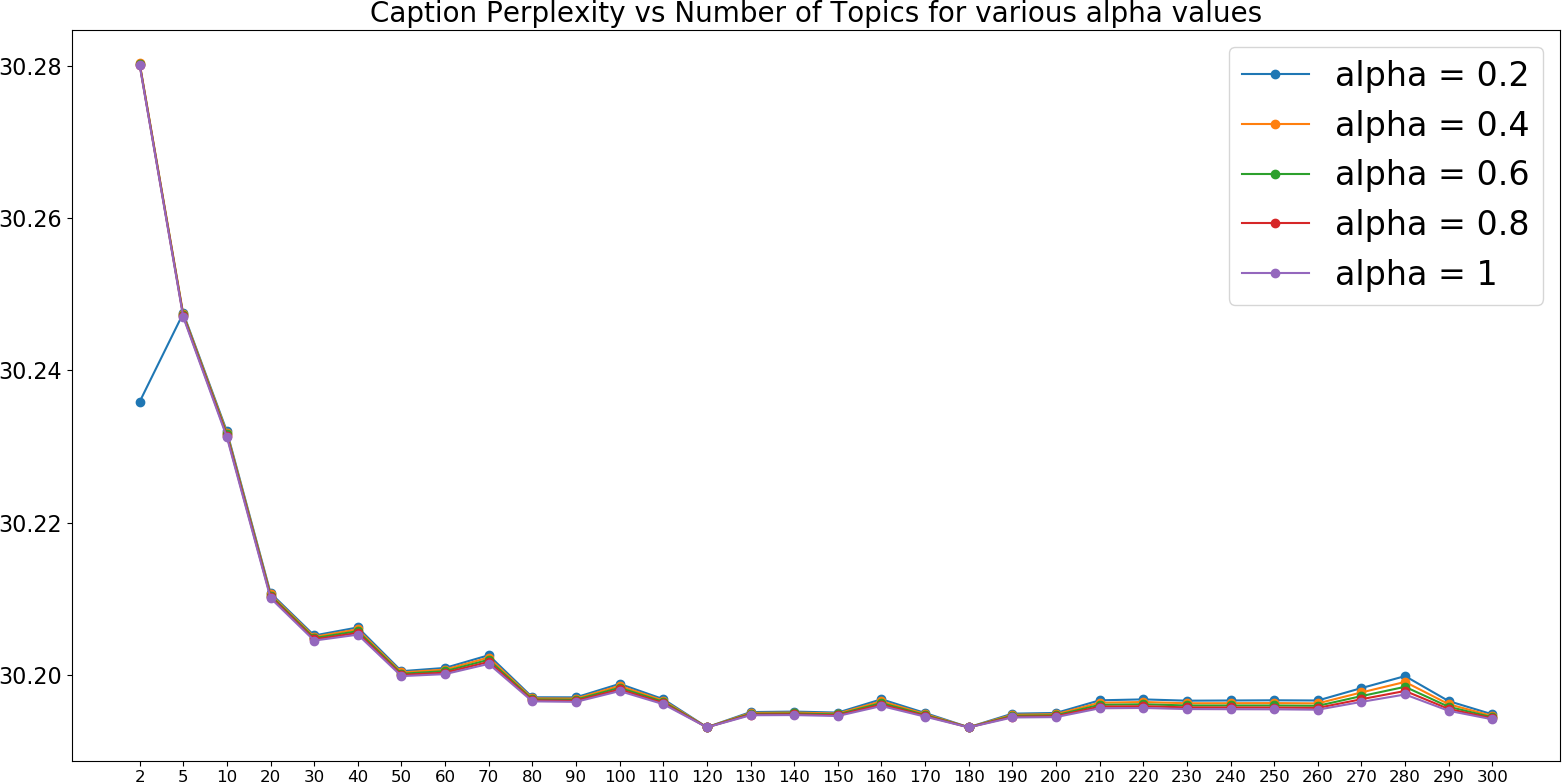
\includegraphics[width=0.45\textwidth]{images/alpha_var1.png}}%
\qquad
\subfigure[Varying values of $\gamma$ for Corel-5k dataset]{%
\label{fig:gamma}%
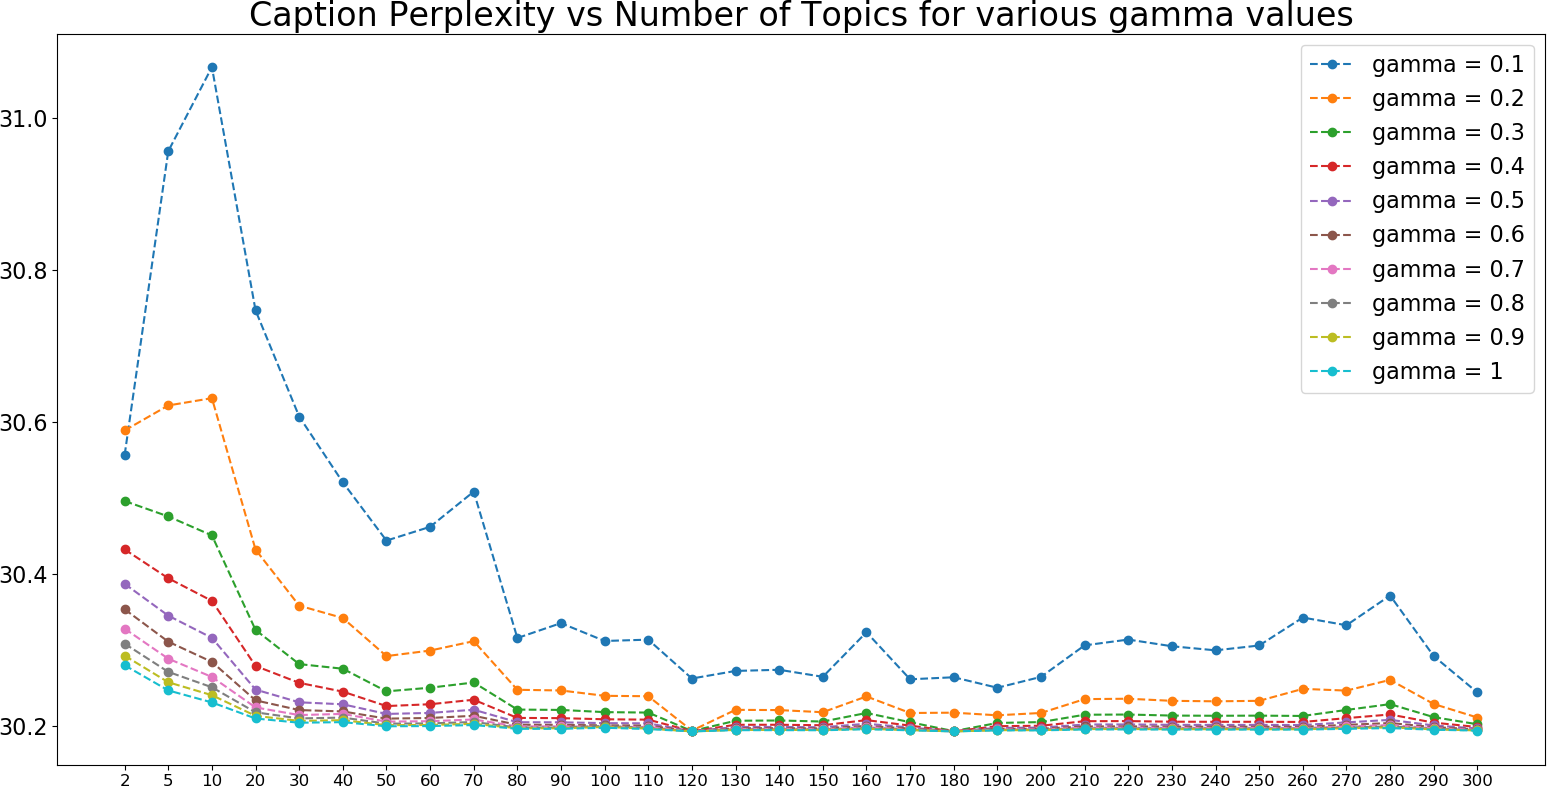
\includegraphics[width=0.45\textwidth]{images/gamma_10.png}}%
\caption{Change in caption perplexity vs number of topics for Corel-5k dataset}
\end{figure*}


\section{Experiments}
The experiments were performed on 3 different datasets so as to compare the performace of code across various kind of SIFT features. This is because across the datasets SIFT features can have an inter-dataset variations apart from the intra-dataset variations. 

\begin{figure}
    \centering
    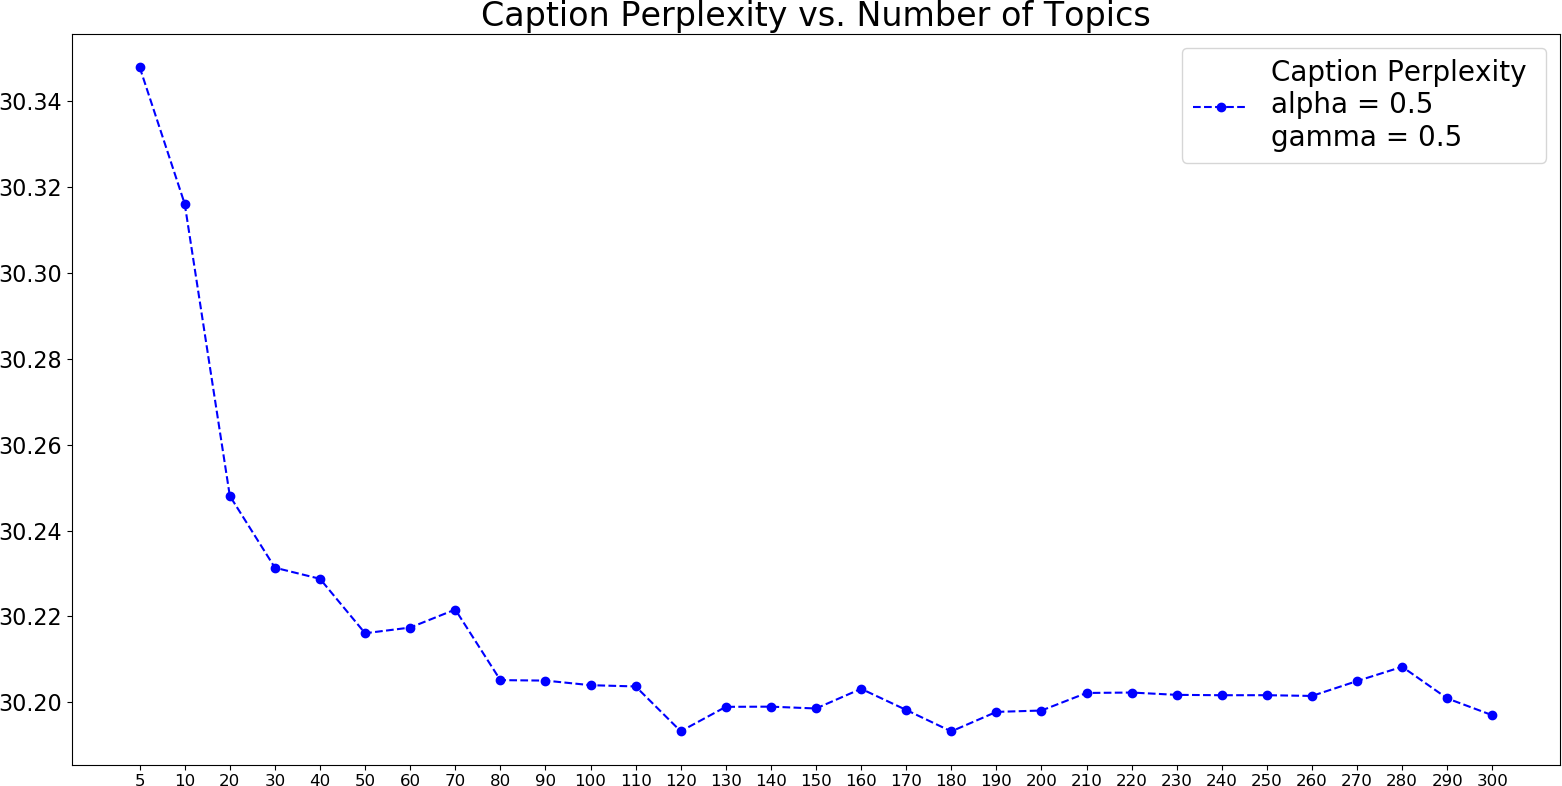
\includegraphics[width=\columnwidth]{images/data1_alpha_05_gamma_05.png}
    \caption{Change in perplexity vs number of topics for Corel-5k dataset. $\alpha = 0.5 $, and $\gamma = 0.5$ were used.}
    \label{fig:c5k}
\end{figure}


\begin{figure}
    \centering
    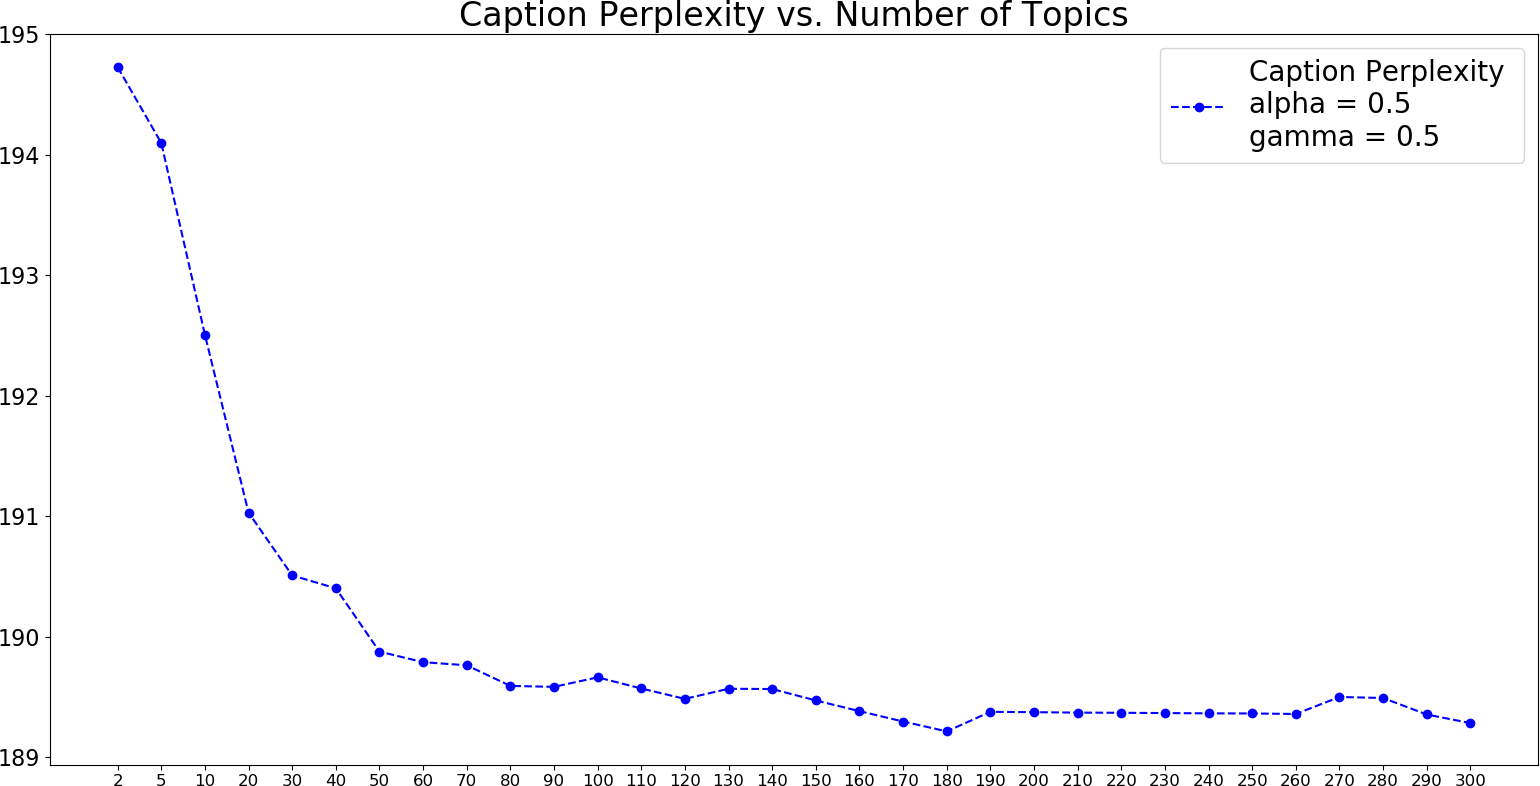
\includegraphics[width=\columnwidth]{images/data2_alpha_05_gamma_05.png}
    \caption{Change in perplexity vs number of topics for MIR flickr dataset. $\alpha = 0.5 $, and $\gamma = 0.5$ were used.}
    \label{fig:mirflickr}
\end{figure}



\begin{figure}
    \centering
    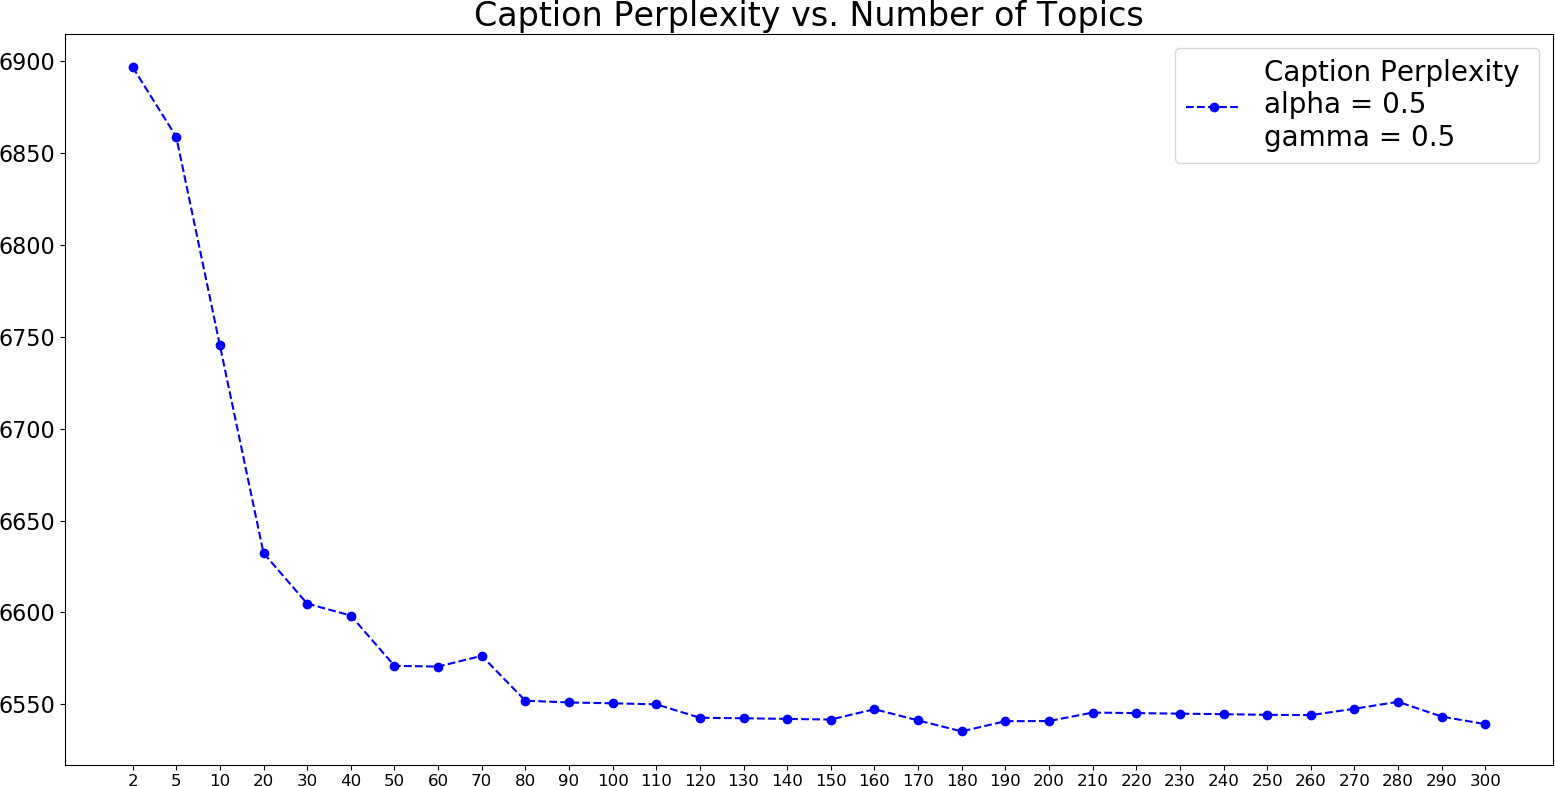
\includegraphics[width=\columnwidth]{images/data3.png}
    \caption{Change in perplexity vs number of topics for ESP game dataset. $\alpha = 0.5 $, and $\gamma = 0.5$ were used.}
    \label{fig:espgame}
\end{figure}

\begin{figure}
    \centering
    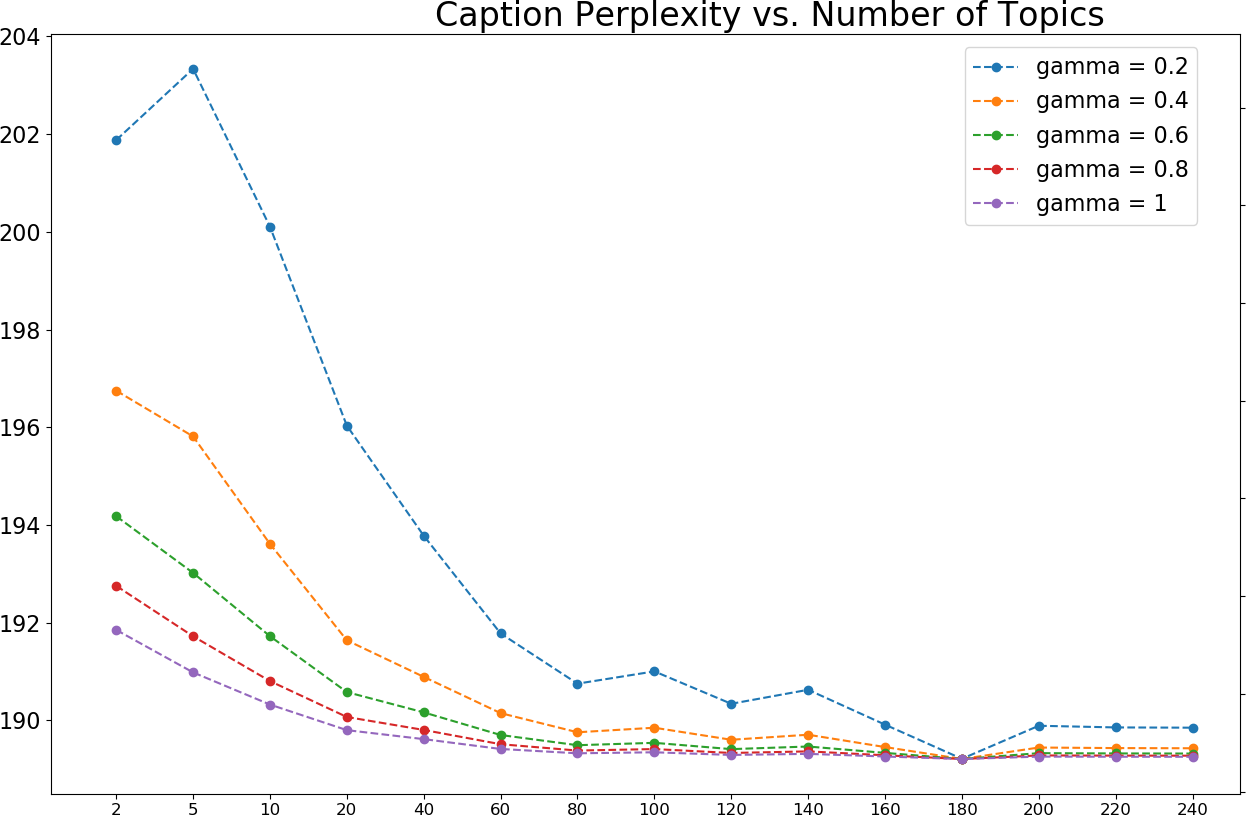
\includegraphics[width=\columnwidth]{images/gamma2.png}
    \caption{Change in perplexity vs number of topics for MIR flickr dataset with $\alpha = 0.5 $, and varying values of $\gamma$}
    \label{fig:gamma2}
\end{figure}

\subsection{Corel-5k dataset}
The Corel-5K dataset \cite{Corel5k}. It has 4999 images, divided into D=4500 training images and 499 test images. There are a total of 371 keywords, with each image being associated with one to five keywords. There are M=260 keywords common between the test and training sets, hence they will be considered for experiments. Each of the N=1000 SIFT feature can be either present in an image or not.

\subsection{MirFlicker dataset}

The MIR flickr dataset \cite{mirflickr}. The dataset contains D = 12500 training images and D = 12500 testing images. After initial processing of data we noticed that many images didn’t have any caption in the dataset.
We cut down those images and shortened test data to D = 9335 and training data to D = 9339 images.
The text vocabulary is M = 457 and N = 1000 SIFT features. The text vocabulary in this dataset is the tags that user put on Flickr when they upload the images.

\subsection{ESP game dataset}
The ESP game dataset \cite{espgame}. It has D=18689 training images and 2081 test images. There are a total of 268 keywords, with each image being associated with one to fifteen keywords. Each of the N=1000 SIFT feature can be either present in an image or not.


The model was also experimented with varying alphas and gammas.


\section{Results}
\subsection{Caption Perplexity}

Perplexity is algebraically equivalent to the inverse of the geometric mean per word likelihood. To measure the annotation quality of the test data set, we computed the perplexity of given caption under $p(w|\mathbf{r})$ for each image in the dataset.
\begin{equation}
    \text{perplexity} = exp \Big\{ \frac{-\sum_{d=1}^{D} \sum_{m=1}^{M_d} log\, p (w_m|\mathbf{r}_d)}{\sum_{d=1}^D M_d}\Big\}
\end{equation}


As the number of topics K is increased, the perplexity drops exponentially as shown in figure \ref{fig:c5k} for Corel-5k dataset, suggesting that the captions are better figured out as they are divided into a lot of topics.
The caption in this dataset are the tags that users put on the flickr images. The reason for perplexity being so high might be because of the fact that users tend to put a lot of tags which are irrelevant with the image content. But still we are able to see the reduction in the caption perplexity as the number of topics are increasing, which in correspondence with the Corel5k dataset where we noticed the similar behaviour.
But after a threshold, the perplexity value starts increasing which depicts that the caption prediction affects with large number of topics 

For the MIR flickr dataset and  ESP game dataset we are showing the variations in the caption perplexity with varying number of topics, the hyperparameters $\alpha$ and $\gamma$ are set to 0.5 and 0.5 respectively. The resulting figures \ref{fig:mirflickr} and \ref{fig:espgame} show the trend similar to the one in corel-5k dataset. The perplexity values go down as we increase the number the topics till a certain threshold. After this threshold point, if we increase the number of topics, the perplexity values increase by a slight number. 

The minimum values achieved for caption perplexity and the corresponding number of topics at which these were observed are shown in table \ref{tab:spet}. It is clear that the range of perplexity values and ideal number of topics vary differently across datasets.

\begin{table}[htb]
    \captionsetup{labelsep=period}
    \centering
    \begin{tabular}{|c|c|c|c|}
        \hline
        & Corel-5k & MIR flickr  & ESP game  \\
        \hline
        Number Of Topics & 120& 180 & 180\\
         \hline
         Caption Perplexity & 30.193261 & 189.213089 & 6535.177535\\
         \hline
    \end{tabular}
    \caption{Number of Topics with least perplexity values for each data-set for $alpha$ = 0.5 $gamma$ = 0.5}
    \label{tab:spet}
\end{table}

\subsection{Varying hyperparameter $\alpha$}
According to \cite{blei2003latent}, changing the hyperparamater $\alpha$ from which we generate $\theta$ for each document assuming dirichlet distribution affects the clustering of topics. Here we don't analyze the clustering of topics, but we are trying to ascertain how it affects the accuracy in terms of caption perplexity as we increase number of topics. 

As we can see in figure \ref{fig:alpha}, the hyperparameter $\alpha$ is not having any considerable effect on the perplexity for the corel-5k dataset. Similar trends were seen for the other 2 datasets.

\subsection{Varying hyperparameter $\gamma$}
As we can see from the figures \ref{fig:gamma}, and \ref{fig:gamma2} corresponding to datasets Corel-5k and MIR flickr dataset, we can see that with low values of $gamma$ the perplexity is high and reduces with  the increase in number of topics.
In few cases we noticed that perplexity values increases for small number of topics and $gamma$, but it eventually decreases as number of topics are increased. This anomalous behavior occurs due to the random initialization of the variables. Similar trends were seen for the other 2 datasets.

\section{Conclusion}
The Corr-LDA model was implemented and tested successfully on various data-sets.
We calculated caption perplexity, which denotes the annotation quality, and noticed that the perplexity is high for small number of topics and reduces as number of topics are increased. The perplexity starts increasing if number of topics is too high. This threshold of number of topics is different for different data-sets. The perplexity values vary across data-sets. This is probably because of the accuracy of the caption given to image. For the accurate captions in Corel5k data-set, the caption perplexity was less, but for the tags in MIRFLICKR data-set, the perplexity was high. Hence we can say that number of topics at which the perplexity is the lowest can describe data most efficiently.
Corr-LDA provides a clean probabilistic model to describe the multi-type data such as images and their captions.

\section{Future Work}
As discussed in the paper \cite{futureWork}, we can use seeds for the topics for a better perplexity, increasing the accuracy of caption prediction.
We can provide a set of seeds words that we believe to be representative of that given data. 
The seed words can bias the topics to improve topic-word distribution. Also they can bias the documents to select the topics related to the seed words and hence improve document-topic distributions.
This approach would result into a better perplexity as seed words can direct the probability distributions away from errors.


\section*{Acknowledgment}
The authors would like to thank \textit{Dr. Hemanth Venkateswara}, and \textit{Ms. Yuzhen Ding} for mentoring this project.

\balance
\bibliographystyle{IEEEtran}
\bibliography{topic_modeling}

\end{document}


